

\begin{abstract} 
Consider the expected query complexity of computing the $k$-fold direct product $f^{\otimes k}$ of a function $f$ to error $\varepsilon$ with respect to a distribution $\mu^k$. One strategy is to sequentially compute each of the $k$ copies to error $\varepsilon/k$ with respect to $\mu$ and apply the union bound. We prove a {\sl strong direct sum theorem} showing that this naive strategy is essentially optimal. In particular, computing a direct product necessitates a blowup in both query complexity {\sl and} error. 

Strong direct sum theorems contrast with results that only show a blowup in query complexity or error but not both. There has been a long line of such results for distributional query complexity, dating back to (Impagliazzo, Raz, Wigderson 1994) and (Nisan, Rudich, Saks 1994), but a strong direct sum theorem had been elusive.

%\gray{ Strong direct sum theorems contrast with weak ones, which only show a blowup in query complexity or error, but not both. There has been a long line of work on strong and weak direct sum theorems for distributional query complexity, dating back to (Impagliazzo, Raz, Wigderson 1994) and (Nisan, Rudich, Saks 1994), but a strong direct sum theorem that holds for all functions in the standard query model had been elusive. } 

A key idea in our work is the first use of the Hardcore Theorem (Impagliazzo 1995) in the context of query complexity. We prove a new ``resilience lemma" that accompanies it, showing that the hardcore of $f^{\otimes k}$ is likely to remain dense under arbitrary partitions of the input space. 


%In addition to our main result, we also (i) prove an equivalence between direct product theorems and XOR lemmas for query complexity, thereby unifying previous works on these problems (Drucker 2012; Blais and Brody 2019; Brody et al.~2022); (ii) suggest an approach towards strong direct product theorems and XOR lemmas for boolean circuits, longstanding open problems of complexity theory; (iii) show implications of our result for boosting in learning theory.
\end{abstract} 

\thispagestyle{empty}

\newpage 
 \setcounter{tocdepth}{2}
\tableofcontents
\thispagestyle{empty}

\newpage 

\setcounter{page}{1}


\section{Introduction}


The {\sl direct sum problem} seeks to understand the ways in which the complexity of solving~$k$ independent instances of a computational task scales with~$k$. This problem and its variants such as the {\sl XOR problem}, where one only seeks to compute the XOR of the $k$ output values, have a long history in complexity theory.  Research on them dates back to Strassen~\cite{Str73} and they have since been  studied in all major computational models including boolean circuits~\cite{Yao82,Lev85,GNW11,Imp95,IW97,OD02,IJKW08,Dru13}, communication protocols~\cite{IRW94,Sha04,KSdW07,LSS08,VW08,Kla10,She11,Jai15,JPY12,BBCR10,BRWY13,Yu22}, as well as classical~\cite{IRW94,NRS94,Sha04,KSdW07,Dru12,BDK18,BB19,BKLS23,Hoza23} and quantum query complexity~\cite{ASdW06,KSdW07,Spa08,She11,AMRR11,LR13}. 

\subsection{This work} 

We focus on classical query complexity, and specifically distributional query complexity. Distributional complexity, also known as average-case complexity, is a basic notion applicable to all models of computation. Direct sum theorems and XOR lemmas for distributional complexity, in addition to being statements of independent interest, have found applications in areas ranging from derandomization~\cite{Yao82,NW94,IW97} to streaming~\cite{AN21} and property testing~\cite{BKST23}.

Let $f: \bn \to \bits$  be a boolean function, $\mu$ be a distribution over $\bn$, and consider the task of computing the $k$-fold direct product $f^{\otimes k}(X^{(1)},\ldots,X^{(k)}) \coloneqq (f(X^{(1)}),\ldots,f(X^{(k)}))$ of $f$ to error $\varepsilon$ with respect to~$\mu^k$. One strategy is to sequentially compute each $f(X^{(i)})$ to error $\varepsilon/k$ with respect to $\mu$ and apply the union bound. Writing $\overline{\mathrm{Depth}}^{\mu}(f,\varepsilon)$ to denote the minimum expected depth of any decision tree that computes $f$ to error $\varepsilon$ w.r.t.~$\mu$, this shows that: %\lnote{Should we change $\overline{\mathrm{Depth}}$ to $\overline{\mathrm{D}}$?}
\begin{equation*}
\overline{\mathrm{Depth}}^{\mu^k}(f^{\otimes k},\varepsilon) \le k \cdot \overline{\mathrm{Depth}}^{\mu}(f,\tfrac{\varepsilon}{k}).
\label{eq:naive upper bound}
\end{equation*}

Our main result is that this naive strategy is essentially optimal for all functions and distributions:\medskip 

\begin{tcolorbox}[colback = white,arc=1mm, boxrule=0.25mm]
\begin{theorem}[Strong direct sum theorem for distributional query complexity; special case of~\Cref{thm:main-formal}]
\label{thm:main-intro}
For every function $f: \bn \to \bits$, distribution $\mu$  over $\bn$, integer $k \in \N$, and $\varepsilon < 1$, 
\[ \overline{\mathrm{Depth}}^{\mu^k}(f^{\otimes k},\varepsilon) \ge \tilde{\Omega}(\eps^2k) \cdot \overline{\mathrm{Depth}}^{\mu}(f,\Theta(\tfrac{\varepsilon}{k})).\]
\end{theorem}
\end{tcolorbox}
\medskip 

Such direct sum theorems are termed {\sl strong}, referring to the fact that they show that computing a direct product necessitates a blowup in {\sl both} the computational resources of interest---in our case, query complexity---{\sl and} error. Strong direct sum theorems contrast with standard ones, which only show a blowup in computational resource, and also with direct {\sl product} theorems, which focus  on the blowup in error. We give a detailed overview of prior work in~\Cref{sec:background}, mentioning for now that while standard direct sum and direct product theorems for distributional query complexity have long been known, a strong direct sum theorem had been elusive.  Prior to our work, it was even open whether 
$\overline{\mathrm{Depth}}^{\mu^k}(f^{\otimes k},1.01\varepsilon) \ge 1.01 \cdot \overline{\mathrm{Depth}}^{\mu}(f,\varepsilon)$ holds. Indeed, the problem is known to be quite subtle, as a striking counterexample of Shaltiel~\cite{Sha04} shows that a strong direct sum
theorem is badly false if one considers {\sl worst-case} instead of expected query complexity. 


\paragraph{A strong XOR lemma.} We also obtain a strong XOR lemma (\Cref{thm:main-xor}) as a corollary of a simple equivalence between direct sum theorems and XOR lemmas for query complexity. One direction is immediate, since the $k$-fold XOR $f^{\oplus k}(X^{(1)},\ldots,X^{(k)}) \coloneqq f(X^{(1)}) \oplus \cdots \oplus f(X^{(k)})$ can only be easier to compute than the $k$-fold direct product.
%\gray{For every function $f:\bn\to\bits$, error parameter $\eps$, and distribution $\mathcal{D}$, the $k$-wise XOR of $f$ defined as $f^{\oplus k}(x)\coloneqq f(x^{(1)})\oplus\cdots\oplus f(x^{(k)})$ satisfies $\overline{\mathrm{Depth}}^{\mu^k}(f^{\otimes k},{\eps})\ge\overline{\mathrm{Depth}}^{\mu^k}(f^{\oplus k},{\eps})$. Therefore, if an XOR lemma of the form $\overline{\mathrm{Depth}}^{\mu^{\oplus k}}(f^{\oplus k},\eps)\ge M\cdot\overline{\mathrm{Depth}}^{\mu}(f,\delta)$ holds, then so does the direct product theorem $\overline{\mathrm{Depth}}^{\mu^k}(f^{\oplus k},\eps)\ge M\cdot\overline{\mathrm{Depth}}^{\mu}(f,\delta)$. We also prove the harder direction, that a strong direct product theorem implies a strong XOR lemma.} 
For the query model we show that the converse also holds: a direct sum theorem implies an XOR lemma with analogous
%\footnote{We say ``analogous" rather than ``the same" because of the additional factor of $\frac1{2}$ on the LHS of the XOR lemma. This factor is necessary since $f^{\oplus k}$ can trivially be computed to error $\frac1{2}$ whereas this is not the case for $f^{\otimes k}$.} 
parameters. %\lnote{Move the statement of the claim (commented out below) to the body. Smooth things over: the title of that subsection will have to change and we'll have to add some prose. }



%%%% MOVE TO BODY %%%%%

 %\begin{claim}
%\label{claim:equivalence between direct product and XOR}
%For every $f:\bn\to\bits$, distribution $\mu$ over $\bn$, integer $k\in\N$, multiplicative factor $M \in \R$, and $\eps\in (0,1)$, if the following direct product theorem holds:
%$$
%\overline{\mathrm{Depth}}^{\mu^k}(f^{\otimes k},\eps)\ge M\cdot\overline{\mathrm{Depth}}^{\mu}(f,\delta).
%$$
%then, the following XOR lemma holds:
%$$
%\overline{\mathrm{Depth}}^{\mu^k}(f^{\oplus k},\tfrac{\eps}{2})\ge M\cdot\overline{\mathrm{Depth}}^{\mu}(f,\delta).
%$$
%\end{claim}



\section{Broader context: Comparison with the randomized setting}
\label{sec:challenges}

Direct sum theorems are also well-studied in the setting of {\sl randomized} query complexity. Recall that the $\eps$-error randomized query complexity of $f$, denoted $\overline{\mathrm{R}}(f,\eps)$, is the minimum expected depth of any randomized  decision tree that computes $f$ with error at most $\eps$ for all inputs.  By Yao's minimax principle, direct sum theorems for distributional query complexity imply analogous ones for randomized query complexity. However, as we now elaborate, such theorems are substantially more difficult to prove in the distributional setting. 


\subsection{A simple and near-optimal strong direct sum theorem for $\overline{\mathrm{R}}$} 
\label{sec:simple}
For randomized query complexity, proving a strong direct sum theorem with near-optimal parameters requires only two observations. 

\paragraph{Observation \#1.} The first is that a standard direct sum theorem, one without error amplification, easily holds in the distributional setting, and hence the randomized setting as well by Yao's principle:
\begin{equation}
\overline{\mathrm{Depth}}^{\mu^k}(f^{\otimes k},\varepsilon) \ge \Omega(k) \cdot \overline{\mathrm{Depth}}^{\mu}(f,\varepsilon) \quad \text{and therefore} \quad \overline{\mathrm{R}}(f^{\otimes k},\eps) \ge \Omega(k)\cdot \overline{\mathrm{R}}(f,\eps). \label{eq:BDK1} \end{equation} 
The idea is that given a decision tree $T$ of average depth $q$ that computes $f^{\otimes k}$ with error~$\eps$, one can extract a decision tree of average depth $q/k$ that computes $f$ to error $\eps$:  place the input in a random block $\boldsymbol{i}\sim [k]$, fill the remaining blocks with independent random draws from $\mu$, and return the $\boldsymbol{i}$th bit of $T$'s output. It is straightforward to show that this reduces the average depth of $T$ by a factor of $k$ while preserving its error. 

\paragraph{Observation \#2.} The second observation is standard error reduction of randomized algorithms by repetition,  which in particular implies:  
\begin{equation} \overline{\mathrm{R}}(f, \lfrac{\eps}{k}) \leq O\paren*{\log k}\cdot \overline{\mathrm{R}}(f,\eps).\label{eq:success-amplification}
\end{equation} 
Combining~\Cref{eq:BDK1,eq:success-amplification} yields a strong direct sum theorem
\begin{equation*}
    \overline{\mathrm{R}}(f^{\otimes k}, \eps) \geq \Omega\paren*{\frac{k}{\log k}} \cdot \overline{\mathrm{R}}(f,\tfrac{\eps}{k})\label{eq:easy}
\end{equation*}
that is within a $O(\log k)$ factor of optimal.  

\paragraph{Blais--Brody.} Using more sophisticated techniques, Blais and Brody \cite{BB19} were recently able remove to this $O(\log k)$ factor and obtain an optimal strong direct sum theorem for $\overline{\mathrm{R}}$. Building on their work, Brody, Kim, Lerdputtipongporn, and Srinivasulu~\cite{BKLS23} then obtained an optimal strong XOR lemma for $\overline{\mathrm{R}}$. 


% We remark that the above outline for a direct sum theorem in the randomized model uses generic arguments that apply to many other models of computation. Both Yao's lemma and boosting hold for all reasonable models of computation, and the ``random-block" argument holds for any model that shrinks appropriately under random restrictions.






\subsection{Error reduction fails in the distributional setting} 

While the crux of~\cite{BB19} and~\cite{BKLS23}'s works is the removal of a $O(\log k)$ factor, the situation is very different in the distributional setting. As mentioned, prior to our work even a direct sum theorem where both factor-of-$\tilde{\Omega}(k)$ blowups in~\Cref{thm:main-intro} are replaced by 1.01 was not known to hold. 


With regards to the argument above, it is Observation \#2 that breaks in the distributional setting---not only does error reduction by repetition break, the distributional analogue of~\Cref{eq:success-amplification} is simply false. This points to a fundamental difference between distributional and randomized complexity: while generic error reduction of randomized algorithms is possible in all reasonable models of computation, the analogous statement for distributional complexity is badly false in all reasonable models of computation. For the query model specifically, in~\Cref{sec:no-boosting} we give an easy proof of the following: 

\begin{fact}
    \label{fact:no-boosting}
    For any $n \in \N$ and $\mu$ being the uniform distribution over $\bits^n$, there is a function $f:\bits^n \to \bits$ such that $\overline{\mathrm{Depth}}^{\mu}(f,\tfrac{1}{4}) = 0$ and yet $\overline{\mathrm{Depth}}^{\mu}(f,\tfrac{1}{8}) \geq \Omega(n).$
\end{fact}


\subsection{A brief summary of our approach}
We revisit Observation \#1 and show how the very same extraction strategy can in fact yield a tree with error $\Theta(\eps/k)$, instead of~$\eps$, at the expense of only a slight increase in depth.  A key technical ingredient in our analysis is {\sl Impagliazzo's Hardcore Theorem}~\cite{Imp95}. For intuition as to why this theorem may be relevant for us, we note that it is tightly connected to the notion of {\sl boosting} from learning theory---they are, in some sense, dual to each other~\cite{KS03}. And boosting is, of course, a form of error reduction, albeit one that is more intricate than error reduction by repetition. 

See~\Cref{sec:tech-overview} for a detailed overview of our approach, including a discussion of why Impagliazzo's Hardcore Theorem, as is, does not suffice, thereby necessitating our new ``resilience lemma" that accompanies it.  


    
\section{Prior Work}
\label{sec:background}

We now place~\Cref{thm:main-intro} within the context of prior work on direct sum and product theorems for distributional query complexity. This is a fairly large body of work that dates back to the 1990s. 

\subsection{Standard direct sum and product theorems}

\paragraph{Standard direct sum theorems.} 

As we sketched in~\Cref{sec:simple}, a simple argument shows that 
\begin{equation}
\overline{\mathrm{Depth}}^{\mu^k}(f^{\otimes k},\varepsilon) \ge \Omega(k) \cdot \overline{\mathrm{Depth}}^{\mu}(f,\varepsilon). \label{eq:BDK}
\end{equation} 
This along with an application of Markov's inequality yields: 
\begin{equation}
\mathrm{Depth}^{\mu^k}(f^{\otimes k},\varepsilon-\varepsilon') \ge \Omega(\varepsilon'k)\cdot \mathrm{Depth}^{\mu}(f,\varepsilon),    \label{eq:JKS}
\end{equation}
where $\mathrm{Depth}^{\mu}(\cdot ,\cdot)$ is the analogue of $\overline{\mathrm{Depth}}^{\mu}(\cdot,\cdot)$ for worst-case instead of expected query complexity. (The details of these arguments are spelt out in~\cite{JKS10,BDK18}.) 



Note that the error budget is the same on both sides of~\Cref{eq:BDK} and the error budget on the RHS of~\Cref{eq:JKS} is {\sl larger} than that of the LHS. In a strong direct sum theorem one seeks a lower bound even when the error budget on the RHS is much smaller than that of the LHS, ideally by a multiplicative factor of $k$ to match the naive upper bound.


\paragraph{A direct product theorem.} Impagliazzo, Raz, and Wigderson~\cite{IRW94} proved a direct product theorem which focuses on the blowup in error.  They showed that: 
\begin{equation} \mathrm{Depth}^{\mu^k}(f^{\otimes k},\varepsilon) \ge  \mathrm{Depth}^{\mu}(f,\tfrac{\varepsilon}{k}).\label{eq:IRW}
\end{equation}
While this result has the sought-for factor of $k$ difference between the error budgets on the LHS and RHS, it comes at the price of there no longer being {\sl any} blowup in depth. 
 
% Note that RHS of~\Cref{eq:IRW} is missing a multiplicative factor, ideally $\Omega(k)$, that one seeks in a strong direct sum theorem.  %Put differently, this lower bound is a factor of $k$ off from the naive upper bound (\Cref{eq:naive upper bound}). 


%\paragraph{Standard direct sum theorems.} 

%As we sketched in~\Cref{sec:simple}, a simple argument shows that 
%\begin{equation}
%\overline{\mathrm{Depth}}^{\mu^k}(f^{\otimes k},\varepsilon) \ge \Omega(k) \cdot \overline{\mathrm{Depth}}^{\mu}(f,\varepsilon). \label{eq:BDK}
%\end{equation} 
%This along with an application of Markov's inequality yields: 
%\begin{equation}
%\mathrm{Depth}^{\mu^k}(f^{\otimes k},\varepsilon-\varepsilon') \ge \Omega(\varepsilon'k)\cdot \mathrm{Depth}^{\mu}(f,\varepsilon).    \label{eq:JKS}
%\end{equation}
%(The details of these arguments are spelt out in~\cite{JKS10,BDK18}.) 

%While these results have the sought-for factor of $\Omega(k)$ that is missing on the RHS of~\cite{IRW94}'s result, they come at the price of the error budget being the same on both sides of~\Cref{eq:BDK} and the error budget on the RHS of~\Cref{eq:JKS} being {\sl larger} than that of the LHS. In a strong direct sum theorem one seeks a lower bound even when the error budget on the RHS is much smaller than that of the LHS, ideally by a multiplicative factor of $k$ to match the naive upper bound.

  


\subsection{Progress and barriers towards a strong direct sum theorem}


These results naturally point to the problem of proving a unifying strong direct sum theorem. We now survey efforts at such a best-of-both-worlds result over the years. 

\paragraph{Decision forests.} Nisan, Rudich, and Saks~\cite{NRS94} proved the following strengthening of~\cite{IRW94}’s result. While~\cite{IRW94} gives an upper bound on the success probability of a {\sl single} depth-$d$ decision tree for $f^{\otimes k}$,~\cite{NRS94} showed that the same bound holds even for {\sl decision forests} where one gets to construct a different depth-$d$ tree for each of the $k$ copies of $f$.     

Since one can always stack the $k$ many depth-$d$ trees in a decision forest to obtain a single tree of depth~$kd$,~\cite{NRS94}'s result establishes a special case of a strong direct sum theorem under a structural assumption on the tree for $f^{\otimes k}$. See~\Cref{fig:stacked} in~\Cref{app:figures} for an illustration of the stacked decision tree that one gets from a decision forest. 



\paragraph{Fair decision trees.} Building on the techniques of~\cite{NRS94}, Shaltiel~\cite{Sha04} proved a strong direct sum theorem under a different structural assumption on the tree for $f^{\otimes k}$. He considered decision trees of depth $kd$ that are “fair” in the sense that every path queries each of the $k$ blocks of variables at most $d$ times. (\cite{Sha04} actually proved a strong XOR lemma for fair decision trees, which implies a strong direct sum theorem for such trees.) See~\Cref{fig:fair} in~\Cref{app:figures} for an illustration of a fair decision tree. 

% \begin{center}
% Figure of a fair tree
% \end{center}


\paragraph{Shaltiel's counterexample for worst-case query complexity.}

These results of~\cite{NRS94} and~\cite{Sha04} could be viewed as evidence in favor of a general strong direct sum theorem, one that does not impose any structural assumptions on the tree for $f^{\otimes k}$. However, in the same paper Shaltiel also presented an illuminating example: he constructed a function, which we call $\mathsf{Shal}$, and a distribution $\mu$ such that for all $k\in \N$,%\gnote{I think this example should hold for any $k$? We might want to say that. Also I'm not sure if this is for any $\eps$, or fixing $\eps$ as a constant.} 
%\[ 
%\mathrm{Depth}^{\mu^k}(\mathsf{Shal}^{\otimes k},2^{-C\delta k}) \le O\big(\delta k \cdot \mathrm{Depth}^{\mu}(\mathsf{Shal},\delta)\big)
%\] 
%for all sufficiently large constants $C$. Importantly, the multiplicative factor on the RHS is $\delta k$ instead of $k$. Consequently, by choosing $\delta = \varepsilon/k$ we get:  
\begin{equation} 
\mathrm{Depth}^{\mu^k}(\mathsf{Shal}^{\otimes k},\varepsilon) \le O\big(\mathrm{Depth}^{\mu}(\mathsf{Shal},\tfrac{\varepsilon}{k})\big).
\label{eq:shaltiel}
\end{equation}
This shows, surprisingly, that for {\sl worst-case} query complexity, the factor-of-$\Omega(k)$ blowup in query complexity that one seeks in a strong direct sum theorem is not always necessary, and in fact sometimes even a constant factor suffices. 

\paragraph{Shaltiel's counterexample vs.~\Cref{thm:main-intro}.} This counterexample for worst-case query complexity should be contrasted with our main result,~\Cref{thm:main-intro}, which shows that a strong direct sum theorem holds for {\sl expected} query complexity. 
%We view~\Cref{thm:main-intro} as confirming a remark that Shaltiel made in his paper, that his counterexample ``seems to exploit defects in the formulation of the problem rather than show that our general intuition for direct product assertions is false."\gnote{I really like including this quote} 
Indeed, the starting point of our work was the encouraging observation that Shaltiel's function does in fact satisfy a strong direct sum theorem if one instead considers expected query complexity. That is, for any $\eps < 1$ and sufficiently large $k$,
\[ \overline{\mathrm{Depth}}^{\mu^k}(\mathsf{Shal}^{\otimes k},\varepsilon) \ge \Omega(k) \cdot\overline{\mathrm{Depth}}^{\mu}(\mathsf{Shal},\tfrac{\eps}{k}).\]
This is a simple observation but appears to have been overlooked. As we now overview, subsequent work considered other ways of sidestepping Shaltiel's counterexample. 

%(A different choice of $\delta$ yields

%$$
%\mathrm{Depth}^{\mu^k}(f^{\otimes k},\varepsilon) %\le O\big(\log k\cdot \mathrm{Depth}^{\mu}(f,\varepsilon)\big),
%$$
%showing *no* blowup in error at the cost of only a $O(\log k)$ blowup in query complexity. This implies that the $\varepsilon'$ factor in [BDK16]’s result […] is actually necessary, and that their result […] does not hold for worst-case query complexity.)


\subsection{Results in light of Shaltiel's counterexample}

\paragraph{A strong direct sum theorem for the OR function.} Klauck, {\v{S}}palek, and de Wolf~\cite{KSdW07} sidestepped Shaltiel’s counterexample by considering a {\sl specific} function (and distribution): motivated by applications to time-space tradeoffs, they proved a strong direct sum theorem for the OR function and with $\mu$ being its canonical hard distribution. Using this, they also showed, for all functions $f$ a lower bound on $f^{\otimes k}$'s query complexity in terms of $f$’s block sensitivity. This stands in contrast to a strong direct sum theorem where one seeks a lower bound on $f^{\otimes k}$'s query complexity in terms of~$f$’s query complexity. 


\paragraph{A phase transition in Shaltiel's counterexample.} 
The precise parameters of Shaltiel's counterexample are:
\[ 
\mathrm{Depth}^{\mu^k}(\mathsf{Shal}^{\otimes k},e^{-\Theta(\delta k)}) \le C\delta k \cdot \mathrm{Depth}^{\mu}(\mathsf{Shal},\delta)
\] 
for all sufficiently large constants $C$. Importantly, the multiplicative factor on the RHS is only $\delta k$ instead of $k$, and therefore becomes a constant if the initial hardness parameter is $\delta = \varepsilon/k$ (thereby yielding~\Cref{eq:shaltiel}).    


Drucker~\cite{Dru12} showed that there is a ``phase transition" in Shaltiel’s counterexample in the following sense: for all functions $f$ and a sufficiently small constant $c > 0$, 
\begin{equation}
\mathrm{Depth}^{\mu^k}(f^{\otimes k},1-e^{-\Theta(\delta k)}) \ge c\delta k \cdot \mathrm{Depth}^{\mu}(f,\delta).
\label{eq:drucker}
\end{equation}
Therefore, while~\cite{Sha04} showed the existence of a function $\mathsf{Shal}$ such that its $k$-fold direct product can be computed to surprisingly low error if the depth budget is $C\delta k\cdot \mathrm{Depth}^{\mu}(f,\delta)$ for a sufficiently {\sl large} constant $C$,~\cite{Dru12} showed that for all functions $f$, this stops being the case if the depth budget is instead $c\delta k\cdot \mathrm{Depth}^{\mu}(f,\delta)$ for a sufficiently {\sl small} constant $c$.


\paragraph{Query complexity with aborts.} Blais and Brody~\cite{BB19} showed that Shaltiel's counterexample can be sidestepped in a different way. En route to proving their strong direct sum theorem for randomized query complexity (discussed in~\Cref{sec:challenges}), they considered decision trees $T: \bn \to \{\pm 1,\bot\}$ that are allowed to output $\bot$ (``abort") on certain inputs, and where the error of $T$ in computing a function $f: \bn \to \bits$ is measured with respect to $T^{-1}(\{\pm 1\})$. In other words, $T$’s output on $x$ is considered correct if $T(x) = \bot$. 

Writing $\mathrm{Depth}^{\mu}_{\Pr[\bot]\le\frac1{3}}(f,\varepsilon)$ to denote the minimum depth of any decision tree for $f$ that aborts with probability at most $1/3$ and otherwise errs with probability at most $\varepsilon$ (both w.r.t.~$\mu$),~\cite{BB19} proved that 
\begin{equation}
\mathrm{Depth}^{\mu^k}_{\Pr[\bot]\le\frac1{3}}(f^{\otimes k},\varepsilon) \ge \Omega(k) \cdot \mathrm{Depth}^{\mu}_{\Pr[\bot]\le\frac1{3}}(f,\tfrac{\varepsilon}{k}).
\label{eq:blais brody}
\end{equation}


Even though the error budget on non-aborts is only $\eps/k$ on the RHS, the fact that the tree is allowed to abort with probability $1/3$ means that it is deemed correct on a $1/3$ fraction of inputs ``for free". A decision tree that aborts with probability $1/3$ and otherwise errs with probability $\eps/k$ can therefore be much smaller than one that never aborts and errs with probability $\eps/k$, and indeed, it is easy to construct examples witnessing the maximally large separation: 
\[ 
n = \mathrm{Depth}^{\mu}(f,\tfrac{\varepsilon}{k})  \gg \mathrm{Depth}^{\mu}_{\Pr[\bot]\le\frac1{3}}(f,\tfrac{\varepsilon}{k}) = 1.
\] 



Building on~\cite{BB19}, Brody, Kim, Lerdputtipongporn, and Srinivasulu~\cite{BKLS23} proved a strong XOR lemma for this model of query complexity with aborts, achieving analogous parameters.  

\paragraph{A strong XOR lemma assuming hardness against all depths.}
A standard strong XOR lemma states that if $f$ is hard against decision trees of certain {\sl fixed} depth $d$, then $f^{\otimes k}$ is much harder against decision trees of depth $\Omega(dk)$. Recent work of Hoza~\cite{Hoza23} shows that Shaltiel's counterexample can be sidestepped if one allows for the stronger assumption that $f$'s hardness ``scales nicely" with $d$. (See the paper for the precise statement of the resulting strong XOR lemma.) 


\subsection{Summary}

Summarizing, prior work on direct sum and product theorems for distributional query complexity either: focused on the blowup in error~\cite{IRW94} or query complexity~\cite{JKS10, BDK18}  but not both; considered restrictions (fair decision trees~\cite{Sha04}) or variants (decision forests~\cite{NRS94}; allowing for aborts~\cite{BB19, BKLS23}) of the query model; focused on specific functions (the OR function~\cite{KSdW07}); or imposed additional hardness assumptions about the function~\cite{Hoza23}. \Cref{thm:main-intro}, on the other hand, gives a strong direct sum theorem that holds for all functions in the standard query model. See~\Cref{table}. %\gnote{Nice table!}%\calnote{Maybe put first two rows at the bottom of the table so there's a clear division between ``non-standard'' models which obtain 2 checks and standard models which fail to obtain both checks?}
\medskip 


\begin{table}[ht]
\captionsetup{width=.9\linewidth}
\renewcommand{\arraystretch}{1.9}
\centering
\begin{tabular}{|c|c|c|c|}
\hline
 ~~~Reference~~~ &  \begin{tabular}{c} Error \vspace{-12pt} \\ ~~Amplification~~ \end{tabular} &  \begin{tabular}{c} Query \vspace{-12pt} \\ ~~Amplification~~ \end{tabular}  & \begin{tabular}{c} Query model/ \vspace{-10pt} \\
 Assumption \end{tabular} 
 \\
\hline 
\hline 
~~\cite{JKS10,BDK18}~~ & $\times$ & $\checkmark$ & Standard query model  \\ \hline 
\cite{IRW94} & $\checkmark$ & $\times$ & Standard query model \\ \hline 
\hline 
\cite{NRS94} & $\checkmark$ & $\checkmark$ & Decision forests \\ \hline 
\cite{Sha04} & $\checkmark$ & $\checkmark$ &~~~Fair decision trees~~~\\ \hline 
\cite{KSdW07} & $\checkmark$ & $\checkmark$ & $f = \mathrm{OR}$ \\ \hline 
\cite{BB19,BKLS23} & $\checkmark$ & $\checkmark$ & ~~Decision trees with aborts~~ \\ \hline 
\cite{Hoza23} & $\checkmark$ & $\checkmark$ & ~~Hardness against all depths~~ \\ \hline \hline 
\Cref{thm:main-intro} & $\checkmark$ & $\checkmark$ & Standard query model \\ \hline 
\end{tabular} 
\caption{Direct sum and product theorems for distributional query complexity}
\label{table} 
\end{table} 


\section{Formal statements of our results and their tightness}

\Cref{thm:main-intro} is a special case of the following result: 

\begin{theorem}[Strong direct sum theorem]
\label{thm:main-formal} 
For every function $f: \bn \to \bits$, distribution $\mu$  over $\bn$, $k\in \mathbb{N}$, and $\gamma, \delta \in (0,1)$, we have that 
\[ 
 \overline{\mathrm{Depth}}^{\mu^k}(f^{\otimes k},1-e^{-\Theta(\delta k)}-\gamma) \ge \Omega\left( \frac{\gamma^2 k}{\log(1/\delta)}\right) \cdot \overline{\mathrm{Depth}}^{\mu}(f,\delta).
\] 
\end{theorem} 
We in fact prove a strong {\sl threshold} direct sum theorem which further generalizes~\Cref{thm:main-formal}: while a direct sum theorem shows that $f^{\otimes k}$ is hard to compute, i.e.~it is hard to get {\sl all} $k$ copies of $f$ correct, a threshold direct sum theorem shows that it is hard even to get {\sl most} of the $k$ copies of $f$ correct. See~\Cref{thm:threshold-DPT}. 

By the equivalence between strong direct sum theorems and strong XOR lemmas (\Cref{claim:equivalence between direct product and XOR}), we also get: 

\begin{theorem}[Strong XOR lemma]
\label{thm:main-xor}
For every function $f:\bits^n\to\bits$ and distribution $\mu$ over $\bits^n$, $k\in\N$, and $\gamma,\delta\in(0,1)$, we have that
    $$
    \overline{\mathrm{Depth}}^{\mu^k}\left(f^{\oplus k},\tfrac{1}{2}(1-e^{-\Theta(\delta k)}-\gamma)\right)\ge {\Omega}\left(\frac{\gamma^2 k}{\log(1/\delta)}\right)\cdot\overline{\mathrm{Depth}}^\mu(f,\delta).
    $$
\end{theorem}

\subsection{Tightness} \Cref{thm:main-formal} amplifies an initial hardness parameter of $\delta = \Theta(1/k)$ to $1-\gamma$ for any small constant~$\gamma$ with a near-optimal overhead of 
\[ \Omega\left(\frac{\gamma^2 k}{\log(1/\delta)}\right) = \Omega\left(\frac{k}{\log k}\right).\]
However, due to the polynomial dependence on $\gamma$, we cannot achieve a final hardness parameter that is exponentially close to $1$ as a function of $k$. We show that this is unavoidable since at least a linear dependence on $\gamma$ is necessary:  

\begin{claim}[Linear dependence on $\gamma$ is necessary]
\label{claim:linear dependence on gamma}
        Let $\mathsf{Par} : \bn\to\bits$ be the parity function and $\mu $ be the uniform distribution over $\bn$. Then for all $\gamma$,
    \[
\overline{\mathrm{Depth}}^{\mu^k}(\mathsf{Par}^{\otimes k}, 1 -\gamma) \leq O(\gamma k) \cdot \overline{\mathrm{Depth}}^\mu(\mathsf{Par}, \tfrac1{4}).
    \]
\end{claim}

The same example shows that a linear dependence on $\gamma$ is likewise necessary in the setting of XOR lemmas.  Determining the optimal polynomial dependence on $\gamma$ in both settings, as well as the necessity of the $\log(1/\delta)$ factor, are concrete avenues for future work. 


%\violet{Finally, we note that we {\sl can} achieve a final hardness parameter that is exponentially close to $1$ if the complexity of $f^{\otimes k}$ is measured with respect to {\sl worst-case} depth instead of {\sl expected} depth: 

%\begin{corollary}
%\label{cor:us+drucker}
%    For every function $f: \bn \to \bits$, distribution $\mu$  over $\bn$, $k\in \mathbb{N}$, and $\delta \in (0,1)$, we have that 
%\[ 
%\mathrm{Depth}^{\mu^k}(f^{\otimes k},1-e^{-\Theta(\delta k)}) \ge \Omega\left( \frac{k}{\log(1/\delta)}\right) \cdot \overline{\mathrm{Depth}}^{\mu}(f,\delta).
%\] 
%\end{corollary}

%\Cref{cor:us+drucker} follows by first using~\Cref{thm:main-formal} to amplify an initial hardness parameter of $\delta$ to a constant, and then using~\cite{Dru12}'s result (\Cref{eq:drucker}) to amplify from a constant to exponentially close to $1$.
%} 
%\gray{ 
%\paragraph{Combining~\Cref{thm:main-formal} with Drucker's result.} 
%In spite of~\Cref{claim:linear dependence on gamma}, we observe that we {\sl can} achieve a resulting hardness parameter that is exponentially close to $1$ if the complexity measure on the LHS of~\Cref{thm:main-formal} is worst-case depth instead of expected depth: 
%$$
%\mathrm{Depth}^{\mu^k}(f^{\otimes k},1-(1-\Omega(\delta))^k) \ge \Omega\left( \frac{k}{\log(1/\delta)}\right) \cdot \overline{\mathrm{Depth}}^{\mu}(f,\delta).
%$$
%This is a simple combination of~\Cref{thm:main-formal} with Drucker's result (\Cref{eq:drucker}): first use~\Cref{thm:main-formal} to amplify from an initial hardness parameter of $\delta$ to a constant $c \in (0,1)$, and then use Drucker's result to amplify from $c$ to exponentially close to $1$. (To elaborate on the second step, we apply~\Cref{eq:drucker} with its $\delta$ being $c$, and use the fact that worst-case query complexity is trivially lower bounded by expected query complexity.) } \lnote{Thinking about not including this.}




\section{Technical Overview for~\Cref{thm:main-formal}} 
\label{sec:tech-overview}

%In this section we highlight the main ideas and technical ingredients that go into our proof of~\Cref{thm:main-formal}. 

\subsection{Hardcore measures and the Hardcore Theorem} 

At the heart of our proof is the notion of a {\sl hardcore measure} and {\sl Impagliazzo’s Hardcore Theorem}~\cite{Imp95}, both adapted to the setting of query complexity.  

\begin{definition}[Hardcore measure for query complexity] 
\label{def:hardcore measure} 
We say that $H : \bn \to [0,1]$ is a {\sl $(\gamma,d)$-hardcore measure for $f : \bn \to \bits$ w.r.t.~$\mu$ of density $\delta$} if:
\begin{enumerate} 
\item $H$'s density is $\delta$: $\ds\Ex_{\bx\sim \mu}[H(\bx)] = \delta$. 
\item $d$-query algorithms achieve correlation at most $\gamma$ with $f$ on $H$:%\gnote{We could add an $= \delta \gamma$ on the r.h.s. of this equation} 
\[ \Ex_{\bx\sim \mu}[f(\bx)T(\bx)H(\bx)] \le \gamma \Ex_{\bx \sim \mu}[H(\bx)] = \gamma \delta.\]
for all decision trees $T$ whose expected depth w.r.t.~$\mu$ is at most $d$.
\end{enumerate}
\end{definition}


\begin{theorem}[Hardcore Theorem for query complexity]
    \label{thm:hardcore theorem for DTs}
For every function $f : \bn\to\bits$, distribution $\mu$ over $\bn$, and $\gamma,\delta > 0$, there exists a $(\gamma,d)$-hardcore measure $H$ for $f$ of density $\delta/2$ w.r.t.~$\mu$ where 
\[ d = \Theta\left(\frac{\gamma^2}{\log(1/\delta)}\right)  \overline{\mathrm{Depth}}^\mu(f,\delta). \]
\end{theorem}

%In words, the Hardcore Theorem states that if $f$ is mildly hard against depth-$D$ decision trees, then there exists a measure $H$ on which $f$ is extremely hard against depth-$d$ decision trees. Note, however, that $d \ll D$. This is a long-recognized downside of this important result that poses challenges when used in the context of {\sl strong} direct product theorems; we will return to this point below. 

The Hardcore Theorem was originally proved, and remains most commonly used, in the setting of circuit complexity where it has long been recognized as a powerful result. (See e.g.~\cite{Tre07}, where it is described as ``one of the bits of magic of complexity theory".) We show in~\Cref{appendix:hardcore} that its proof extends readily to the setting of query complexity to establish~\Cref{thm:hardcore theorem for DTs}.  Despite its importance in circuit complexity and its straightforward extension to query complexity, our work appears to be the first to consider its applicability in the latter setting. 



\begin{remark}
For intuition regarding~\Cref{def:hardcore measure}, note that if $H : \bn \to \zo$ is the indicator of a {\sl set}, the two properties simplify to: 
 $\ds \Prx_{\bx \sim \mu}[\bx \in H] = \delta$ and 
$ \ds \Ex_{\bx\sim \mu}[f(\bx)T(\bx) \mid \bx \in H] \le \gamma$. 
    \end{remark}


    
\subsection{Two key quantities: hardcore density and hardcore advantage at a leaf}

\paragraph{Setup.} For the remainder of this section, we fix a function $f : \bn\to\bits$, distribution $\mu$ over $\bn$, and initial hardness parameter $\delta$ (which we think of as small, close to $0$). Let $T : (\bn)^k \to \bits^k$ be a decision tree that seeks to compute $f^{\otimes k}$ w.r.t.~$\mu^k$.   Our goal is to show that $T$'s error must be large, close to $1$, unless its depth is sufficient large.

\paragraph{Definitions of the hardcore density and hardcore advantage at a leaf.} Let $H : \bn\to [0,1]$ be a $(\gamma,d)$-hardcore measure for $f$ of density $\delta$ w.r.t.~$\mu$ given by~\Cref{thm:hardcore theorem for DTs}.  Each leaf $\ell$ of $T$ corresponds to a tuple of restrictions $(\pi_1,\ldots,\pi_k)$ to each of the $k$ blocks of inputs. We will be interested in understanding, for a random block $\boldsymbol{i}\in [k]$, the extent to which the restricted function $H_{\pi_{\boldsymbol{i}}}$ retains the two defining properties of a hardcore measure: high density and strong hardness. We therefore define: 


\begin{definition}[Hardcore density at $\ell$]
\label{def:hardcore-density}
For $i\in [k]$, the {\sl hardcore density at $\ell$ in the $i$th block} is the quantity: 
\[ \Dens_H(\ell,i)\coloneqq \Ex_{\bX\sim \mu^k}\big[H(\bX^{(i)})\mid \text{$\bX$ reaches $\ell$}\big]. \]
The {\sl total hardcore density at $\ell$} is the quantity $\ds \Dens_H(\ell) \coloneqq \sum_{i =1}^k \Dens_H(\ell,i).$
\end{definition}

See \Cref{fig:hardcore} for an illustration of \Cref{def:hardcore-density}.

\def\centerarc[#1](#2)(#3:#4:#5){ \draw[#1] ($(#2)+({#5*cos(#3)},{#5*sin(#3)})$) arc (#3:#4:#5); }
%% https://tex.stackexchange.com/questions/55068/is-there-a-tikz-equivalent-to-the-pstricks-ncbar-command
\tikzset{
    ncbar angle/.initial=90,
    ncbar/.style={
        to path=(\tikztostart)
        -- ($(\tikztostart)!#1!\pgfkeysvalueof{/tikz/ncbar angle}:(\tikztotarget)$)
        -- ($(\tikztotarget)!($(\tikztostart)!#1!\pgfkeysvalueof{/tikz/ncbar angle}:(\tikztotarget)$)!\pgfkeysvalueof{/tikz/ncbar angle}:(\tikztostart)$)
        -- (\tikztotarget)
    },
    ncbar/.default=0.5cm,
}

\tikzset{round left paren/.style={ncbar=0.5cm,out=120,in=-120}}
\tikzset{round right paren/.style={ncbar=0.5cm,out=60,in=-60}}

\newcommand{\quartercirc}{%
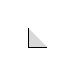
\begin{tikzpicture}
    \centerarc[black,fill=gray!30](0,0)(0:90:0.24);
    \filldraw[fill=gray!30,opacity=0.0,fill opacity=1] (0,0) -- (0,0.24) -- (0.24,0) -- cycle;
    \draw[-] (0,0) to (0,0.24);
    \draw[-] (0,0) to (0.24,0);
\end{tikzpicture}%
}


\begin{figure}[h!]
    \centering
    \begin{tikzpicture}[tips=proper]
        % HOW MUCH TO RIGHT INCREMENT LARGE DENSITY SQUARES
        \def\inc{1.5}
        % HOW MUCH TO RIGHT INCREMENT SMALL DENSITY SQUARES
        \def\sinc{1.2}
        % SIZE OF SMALL DENSITY SQUARES
        \def\s{0.75}
    
        \node[isosceles triangle,
            draw,
            thick,
            isosceles triangle apex angle=60,
            rotate=90,
            minimum size=6cm] (T1) at (0,0){};
        
        \draw[black,dashed] (T1.east) .. controls ([xshift=-0.1cm]T1.358) .. ([yshift=-0.5cm]T1.east) node[] (N1) {{}};
        \draw[black,dashed] ([yshift=-0.5cm]T1.east) .. controls ([xshift=0.4cm]T1.40) and (T1.350) .. (T1.center) node[fill=white,pos=0.9] (N1) {$\pi$};
        \draw[black,dashed] (T1.center) .. controls ([xshift=2.4cm]T1.110) .. (T1.west) node[] (N2) {{}};

        % LOCATION OF TOP HARDCORE DENSITIES
        \coordinate (top) at (5,4);
        \coordinate (top2) at ($(top)+(\inc,0)$); 
        \coordinate (top3) at ($(top2)+(\inc,0)$);
        
        \node[rectangle,
    	draw = black,
    	minimum width = 1cm, 
    	minimum height = 1cm] (r) at (top) {};
        \node[ellipse,
            draw = black,
            fill=gray!30,
            minimum width = 0.4cm,
            minimum height = 0.4cm] (e) at (top) {\footnotesize $H$};
        \node[rectangle,
    	draw = black,
    	minimum width = 1cm, 
    	minimum height = 1cm] (r2) at (top2) {};
        \node[ellipse,
            draw = black,
            fill=gray!30,
            minimum width = 0.5cm,
            minimum height = 0.5cm] (e2) at (top2) {\footnotesize $H$};
        \node[rectangle,
    	draw = black,
    	minimum width = 1cm, 
    	minimum height = 1cm] (r3) at (top3) {};
        \node[ellipse,
            draw = black,
            fill=gray!30,
            minimum width = 0.5cm,
            minimum height = 0.5cm] (e3) at (top3) {\footnotesize $H$};

        % TOP PARENTHESES
        \draw [black] (4.3,3.4) to [round left paren ] (4.3,4.6);
        \draw [black] (8.7,3.4) to [round right paren ] (8.7,4.6);

        % TOP COMMAS
        \draw [black] (5.75,3.5) node [] {\LARGE ,};
        \draw [black] (7.25,3.5) node [] {\LARGE ,};

        % BOTTOM PARENTHESES
        \draw [black] (4.8,-2.5) to [round left paren ] (4.8,-1.5);
        \draw [black] (8.4,-2.5) to [round right paren ] (8.4,-1.5);

        % BOTTOM COMMAS
        \draw [black] (6,-2.4) node [] {\LARGE ,};
        \draw [black] (7.2,-2.4) node [] {\LARGE ,};

        % LOCATION OF BOTTOM HARDCORE DENSITIES
        \coordinate (bot) at (5.4,-2); 
        \coordinate (bot2) at ($(bot)+(\sinc,0)$);
        \coordinate (bot3) at ($(bot2)+(\sinc,0)$);
        
        \node[rectangle,
    	draw = black,
    	minimum width = \s cm, 
    	minimum height = \s cm] (r2) at (bot) {};
        \node[rectangle,
    	draw = black,
    	minimum width = \s cm, 
    	minimum height = \s cm] (r3) at (bot2) {};
        \node[rectangle,
    	draw = black,
    	minimum width = \s cm, 
    	minimum height = \s cm] (r4) at (bot3) {};
       
        \centerarc[black,fill=gray!30]([xshift=-0.38cm,yshift=-0.38cm]bot)(0:90:0.5);
        \centerarc[black,fill=gray!30]([xshift=0.38cm,yshift=0.38cm]bot2)(180:270:0.5);
        \centerarc[black,fill=gray!30]([xshift=0.38cm,yshift=-0.38cm]bot3)(90:180:0.5);

        % FILLING IN LIGHT GRAY REST OF BLOCKS
        \filldraw[fill=gray!30,opacity=0.0,fill opacity=1] (r2.225) -- (r2.162) -- (r2.288) -- cycle;
        \filldraw[fill=gray!30,opacity=0.0,fill opacity=1] (r3.342) -- (r3.45) -- (r3.108) -- cycle;
        \filldraw[fill=gray!30,opacity=0.0,fill opacity=1] (r4.251) -- (r4.315) -- (r4.18) -- cycle;

        % path label
        \draw[color=black] (T1.west) node [below,fill=white] {\footnotesize Leaf $\ell$};
        \node[draw,circle,fill=black,inner sep=1pt] (x) at (T1.west) {};

        % LABELS
        % \draw[-{Stealth[scale=1]}] (6,2.7) to (e);
        % \draw [black] (6,2.7) node [fill=white] {Hardcore measure $H$};

        \draw[-{Stealth[scale=1]}] (4.6,-3.3) to ([xshift=-.2 cm,yshift=-.2cm]bot);
        \draw [black] (4.6,-3.3) node [fill=white] {Hardcore measure $H_{\pi_1}$ with $\mathrm{Dens}_H(\ell, 1)={\mathrm{area}(\quartercirc)}/{\mathrm{area}(\square})$};

        % QUERIES ALONG PATH PI
        \draw[-{Stealth[scale=1]}] (6.5,3) to node[midway,fill=white!30,scale=1] {Queries along path $\pi$} (6.5,-1);

       % REDRAWS
        \node[rectangle,
    	draw = black,
    	minimum width = \s cm, 
    	minimum height = \s cm] (aaaa) at (bot) {};
        \node[rectangle,
    	draw = black,
    	minimum width = \s cm, 
    	minimum height = \s cm] (bbbbb) at (bot2) {};
        \node[rectangle,
    	draw = black,
    	minimum width = \s cm, 
    	minimum height = \s cm] (ccccc) at (bot3) {};
        
    \end{tikzpicture}
    \captionsetup{width=.9\linewidth}
    \caption{Illustration of a hardcore density. The tree $T:(\bn)^3\to\bits^3$ seeks to compute a function $f^{\otimes 3}$. The tuple of squares at the top of the figure illustrates the set of all inputs to the function while the strings in the support of the hardcore measure are shaded gray. The tuple at the bottom of the figure illustrates the set of inputs reaching the leaf $\ell$. Each block is the subcube consistent with the path $\pi$ and the shaded region denotes the fragment of $H$ which is contained in the corresponding subcube. }
    \label{fig:hardcore}
\end{figure}




\begin{definition}[Hardcore advantage at $\ell$]
\label{def:hardcore advantage}
For $i\in [k]$, the {\sl hardcore advantage at $\ell$ in the $i$th block} is the quantity:
\[ \Adv_H(\ell,i) \coloneqq \abs[\Big]{\Ex_{\bX\sim \mu^k}\big[ f(\bX^{(i)})T(\bX)_i H(\bX^{(i)})\mid \text{$\bX$ reaches $\ell$}\big]}.  \]
The {\sl total hardcore advantage at $\ell$} is the quantity  
$ \ds \Adv_H(\ell) \coloneqq \sum_{i=1}^k \Adv_H(\ell, i). $
\end{definition}

% \bigskip

% \begin{center}
% Figure illustrating the two definitions \lnote{Add figure}
% \end{center}

% \bigskip 

Intuitively, leaves for which $\Dens_H(\ell)$ is large and $\Adv_H(\ell)$ is small contribute significantly to error of $T$.~\Cref{lem:accuracy in terms of hardcore density and advantage} below  formalizes this:

\paragraph{Notation} \hspace{-10pt} (Canonical distribution over leaves){\bf .}   We write $\mu^k(T)$ to denote the distribution over leaves of $T$ where:  
\[ \Prx_{\bell\sim \mu^k(T)}[\bell = \ell] = \Prx_{\bX\sim \mu^k}[\text{$\bX$ reaches $\ell$}].\]


\begin{tcolorbox}[colback = white,arc=1mm, boxrule=0.25mm]
\begin{lemma}[Accuracy in terms of hardcore density and advantage at leaves]%\gnote{Changed constant of $2$ to $4$ for proof convenience.}
\label{lem:accuracy in terms of hardcore density and advantage}
\[ 
         \Prx_{\bX \sim \mu^k}[T(\bX) = f^{\otimes k}(\bX)] \leq \Ex_{\bell \sim \mu^k(T)}\bracket*{\exp\paren*{-\frac{\Dens_H(\bell) - \Adv_H(\bell)}{4}}}.
  \] 
\end{lemma} 
\end{tcolorbox}



\subsection{Expected total hardcore density and advantage}


\Cref{lem:accuracy in terms of hardcore density and advantage} motivates understanding the random variables $\mathrm{Dens}_H(\boldsymbol{\ell})$ and $\mathrm{Adv}_H(\boldsymbol{\ell})$ for $\boldsymbol{\ell}\sim \mu^k(T)$. We begin by bounding their expectations:


\begin{claim}[Expected total hardcore density]
\label{claim:expected total hardcore density} If $H$ is a hardcore measure of density $\delta$ then 
\[  \Ex_{\bell\sim \mu^k(T)}[\Dens_H(\bell)] = \delta k. \] 
\end{claim}


\Cref{claim:expected total hardcore density} is a statement about density preservation. It says that $H$'s expected density at a random leaf $\bell \sim \mu^k(T)$ and in a random block $\bi\sim [k]$ is equal to $H$'s initial density: 
\[  \mathop{\Ex_{\bell\sim \mu^k(T)}}_{\bi\sim [k]}\bigg[  \underbrace{\Ex_{\bX\sim \mu^k}\big[H(\bX^{(\bi)})\mid \text{$\bX$ reaches $\bell$}\big]}_{\Dens_H(\bell,\bi)}\bigg] = \delta = \Ex_{\bx\sim \mu}[H(\bX)]. \]
 

\begin{claim}[Expected total hardcore advantage]
\label{claim:expected total hardcore advantage}
    If $H$ is a $(\gamma, d)$-hardcore measure for $f$ of density $\delta$ w.r.t.~$\mu$ and the expected depth of $T$ is at most $dk$, then 
    \begin{equation*}
        \Ex_{\bell \sim \mu^k(T)}[\adv_H(\bell)] \leq \gamma \Ex_{\bell\sim\mu^k(T)}[\Dens_H(\bell)]. 
    \end{equation*}
\end{claim}


\Cref{claim:expected total hardcore advantage} is a statement about depth amplification. By definition, $H$ being a $(\gamma,d)$-hardcore measure for $f$ means that 
    \begin{equation*}
        \underbrace{ \Ex_{\bx \sim \mu}[ f(\bx) T_{\textnormal{small}}(\bx) H(\bx)]}_{\textnormal{Hardcore advantage}}  \leq \gamma  \underbrace{\Ex_{\bx \sim \mu}[H(\bx)]}_{\textnormal{Hardcore density}}
    \end{equation*}
    for every tree $T_{\mathrm{small}} : \bn\to\bits$ of expected depth $d$.~\Cref{claim:expected total hardcore advantage} says that 
\[ \underbrace{\sum_{i=1}^k \Ex_{\bX\sim \mu^k}\big[ f(\bX^{(i)})T_{\textnormal{large}}(\bX)_i H(\bX^{(i)})\big] }_{\textnormal{Total hardcore advantage}} \le  \gamma   \underbrace{\sum_{i=1}^k \Ex_{\bX\sim\mu^k}[H(\bX^{(i)})]}_{ \textnormal{Total hardcore density}}. \]
for every tree $T_{\textnormal{large}} : (\bn)^k \to \bits^k$ of expected depth $dk$. Crucially, the depth of $T_{\textnormal{large}}$ is allowed to be a factor of $k$ larger than that of $T_{\textnormal{small}}$, and yet the ratio of hardcore advantage to hardcore density remains the same ($\gamma$ in both cases).  



\subsubsection{Done if Jensen went the other way}
\label{sec:jensen}
For intuition as to why~\Cref{claim:expected total hardcore density} and~\Cref{claim:expected total hardcore advantage} are relevant yet insufficient for us, note that if it were the case that $\mathbb{E}[\exp(-\boldsymbol{Z})] \le \exp(-\mathbb{E}[\boldsymbol{Z}])$, which unfortunately is the opposite of what Jensen’s inequality gives, we would have the strong bound on the accuracy of $T$ that we seek:   
\begin{align*}
 \Prx_{\bX \sim \mu^k}[T(\bX) = f^{\otimes k}(\bX)] &\leq \Ex_{\bell \sim \mu^k(T)}\bracket*{\exp\paren*{-\frac{\dens_H(\bell) - \adv_h(\bell)}{4}}} \tag{\Cref{lem:accuracy in terms of hardcore density and advantage}} \\
 &``\le" \exp\bigg(- \Ex_{\bell\sim\mu^k(T)}\bigg[\frac{\Dens_H(\bell)-\Adv_H(\bell)}{4}\bigg] \bigg) \tag{Wrong direction of Jensen} \\
 &\le \exp\bigg(-\frac{\delta k -\gamma \delta k}{4} \bigg)  \tag{\Cref{claim:expected total hardcore density} and \Cref{claim:expected total hardcore advantage}} \\
 &\le \exp(-\Theta(\delta k)). 
\end{align*}

For an actual proof, we need to develop a more refined understanding of the distribution of $\mathrm{Dens}_H(\boldsymbol{\ell})$ beyond just its expectation. (As it turns out, this along with the bound on $\mathbb{E}[\mathrm{Adv}_H(\boldsymbol{\ell})]$ given by~\Cref{claim:expected total hardcore advantage} suffices.) 

\subsection{A resilience lemma for hardcore measures}


\paragraph{An illustrative bad case to rule out.} Suppose $T$ were such that it achieved $\mathbb{E}[\mathrm{Dens}_H(\boldsymbol{\ell})] =  \delta k$ by having a $\delta$-fraction of leaves with $\mathrm{Dens}_H(\ell) = k$ and the remaining $1-\delta$ fraction with $\mathrm{Dens}_H(\ell) = 0$. If this were the case then “all the hardness” would be concentrated on a small $\delta$ fraction of leaves, and the best lower bound that we would be able to guarantee on error of $T$ with respect to $f^{\otimes k}$ would only be $\delta$. This is our starting assumption on the hardness of $f$, and so no error amplification has occurred. 

\paragraph{The resilience lemma.} We rule out cases like this by showing that $T$ must achieve $\mathbb{E}[\mathrm{Dens}_H(\boldsymbol{\ell})]=  \delta k$ by having the vast majority of its leaves with $\mathrm{Dens}_H(\ell) = \Omega(\delta k)$, i.e.~that $\Dens_H(\bell)$ is tightly concentrated around its expectation:  
\medskip 

\begin{tcolorbox}[colback = white,arc=1mm, boxrule=0.25mm]
\begin{lemma}[Resilience lemma]
\label{lem:resilience lemma}
For any hardcore measure $H$ of density $\delta$ w.r.t.~$\mu$ and tree $T:(\bn)^k \to \bits^k$,
\begin{equation*}
    \Prx_{\bell \sim \mu^k(T)}[\Dens_H(\bell) \leq \delta k/2] \leq e^{-\delta k/8}.
\end{equation*}
Similarly, $\ds \Prx_{\bell \sim \mu^k(T)}[\Dens_H(\bell) \geq 2\delta k] \leq e^{-\delta k/3}.$ 
\end{lemma}
\end{tcolorbox}
\medskip 

\begin{figure}[H]
\centering
\hspace*{\fill}
\begin{subfigure}{.45\textwidth}
  \centering
  % \resizebox{0.65\textwidth}{!}{%
      \begin{tikzpicture}[tips=proper]
        \node[isosceles triangle,
            draw,
            isosceles triangle apex angle=60,
            rotate=90,
            minimum size=6cm] (T1) at (0,0){};
            
        \draw[black,dashed] (T1.east) .. controls ([xshift=-0.1cm]T1.358) .. ([yshift=-0.5cm]T1.east) node[] (N1) {{}};
        \draw[black,dashed] ([yshift=-0.5cm]T1.east) .. controls ([xshift=0.4cm]T1.40) and (T1.350) .. (T1.center) node[] (N1) {};
        \draw[black,dashed] (T1.center) .. controls ([xshift=2.4cm]T1.110) .. ([xshift=-0.15cm]T1.west) node[] (N2) {{}};
        
        % leaf label
        \draw[-{Stealth[scale=1]}] ([xshift=0.5cm,yshift=0.5cm]T1.west) to ([xshift=-0.15cm]T1.west);
        \draw[] ([xshift=0.5cm,yshift=0.7cm]T1.west) node [right,black,fill=white, text width=2cm] {\footnotesize Leaf $\ell$ with $\mathrm{Dens}_H(\ell)=0$};
        
        % brackets
        % delta-fraction
        \draw [black,decorate,decoration={brace,mirror,raise=1pt,amplitude=3pt}] ([xshift=0.2cm,yshift=-0.5cm]T1.left corner) -- ([xshift=2.8cm,yshift=-0.5cm]T1.left corner) node [black,pos=0.5,yshift=-0.5cm] {\small $\delta$-fraction};

        % 1-delta fraction
        \draw [black,decorate,decoration={brace,mirror,raise=1pt,amplitude=3pt}] ([xshift=3.2cm,yshift=-0.5cm]T1.left corner) -- ([xshift=7.0cm,yshift=-0.5cm]T1.left corner) node [black,pos=0.5,yshift=-0.5cm] {\small $(1-\delta)$-fraction};

        % leaf values
        \draw [] ([xshift=0cm]T1.left corner) -- (T1.right corner) node [black,pos=0.5,below] { $~ k\quad k\quad k\quad k\quad k \quad 0\quad 0\quad 0\quad 0\quad 0\quad 0\quad 0$};   
    \end{tikzpicture}
    % }
  \caption{An illustration of the bad case where $\mathrm{Dens}_H$ is anti-concentrated away from its mean of $\delta k$.}
  \label{fig:bad case}
\end{subfigure}%
\hfill
\begin{subfigure}{.45\textwidth}
  \centering
  % \resizebox{0.65\textwidth}{!}{
          \begin{tikzpicture}[tips=proper]
        \node[isosceles triangle,
            draw,
            isosceles triangle apex angle=60,
            rotate=90,
            minimum size=6cm] (T1) at (0,0){};
            
        \draw[black,dashed] (T1.east) .. controls ([xshift=-0.1cm]T1.358) .. ([yshift=-0.5cm]T1.east) node[] (N1) {{}};
        \draw[black,dashed] ([yshift=-0.5cm]T1.east) .. controls ([xshift=0.4cm]T1.40) and (T1.350) .. (T1.center) node[] (N1) {};
        \draw[black,dashed] (T1.center) .. controls ([xshift=2.4cm]T1.110) .. ([xshift=-0.3cm]T1.west) node[] (N2) {{}};
        
        % leaf label
        \draw[-{Stealth[scale=1]}] ([xshift=0.35cm,yshift=0.5cm]T1.west) to ([xshift=-0.3cm]T1.west);
        \draw[] ([xshift=0.4cm,yshift=0.7cm]T1.west) node [right,black, text width=2.2cm] {\footnotesize Leaf $\ell$ with $\mathrm{Dens}_H(\ell)\approx\delta k$};

        % brackets
        % delta-fraction
        \draw [white,decorate,decoration={brace,mirror,raise=1pt,amplitude=3pt}] ([xshift=0.2cm,yshift=-0.5cm]T1.left corner) -- ([xshift=2.6cm,yshift=-0.5cm]T1.left corner) node [white,pos=0.5,yshift=-0.65cm] {{}};
        
        % leaf values
        \draw [] ([xshift=0cm]T1.left corner) -- (T1.right corner) node [black,pos=0.5,below] { $\approx\delta k~~\approx\delta k~~\approx\delta k~~\approx\delta k~~ \approx\delta k~~ \approx\delta k$\vspace{2em}};
        \end{tikzpicture}
    % }
  \caption{An illustration of the good case where $\mathrm{Dens}_H$ is concentrated around its mean of $\delta k$. }
  \label{fig:good case}
\end{subfigure}
\hspace*{\fill}
  \captionsetup{width=.9\linewidth}
\caption{An illustration of our resilience lemma (\Cref{lem:resilience lemma}). This lemma shows that all trees resemble the one on the right, with $\mathrm{Dens}_H(\bell)$ tightly concentrated around its mean of $\delta k$. This allows us to rule out bad trees such as those on the left where all of the hardness is concentrated on a small fraction of the leaves.}
\label{fig:resilience lemma}
\end{figure}








Comparing~\Cref{lem:resilience lemma} to~\Cref{claim:expected total hardcore advantage}, we see that~\Cref{claim:expected total hardcore advantage} is a statement about density preservation {\sl in expectation} whereas~\Cref{lem:resilience lemma} is a statement about density preservation {\sl with high probability}. It says that $H$'s density at a random leaf $\bell\sim \mu^k(T)$ and in a random block $\bi\sim [k]$ remains, with high probability, roughly the same as that of $H$'s initial density---this is why we call~\Cref{lem:resilience lemma} a resilience lemma. (Our proof of~\Cref{lem:resilience lemma} in fact shows that the $H$'s density remains resilient under arbitrary partitions of $(\{ \pm 1\}^n)^k$, not just those induced by a decision tree.)


With~\Cref{lem:resilience lemma} in hand, the intuition sketched in~\Cref{sec:jensen} can be made formal. 

\section{Discussion and Future Work}

Our main results are a strong direct sum theorem and a strong XOR lemma for distributional query complexity, showing that if $f$ is somewhat hard to approximate with depth-$d$ decision trees, then $f^{\otimes k}$ and $f^{\oplus k}$ are both {\sl much harder} to approximate, even with decision trees of {\sl much larger} depth.  These results hold for expected query complexity, and they circumvent a counterexample of Shaltiel showing that such statements are badly false for worst-case query complexity.  We view our work as confirming a remark Shaltiel made in his paper, that his counterexample ``seems to exploit defects in the formulation of the problem rather than show that our general intuition for direct product assertions is false."


Shaltiel's counterexample applies to  
 many other models including boolean circuits and communication protocols. A broad avenue for future work is to understand how this counterexample can be similarly circumvented in these models by working with more fine-grained notions of computation cost.  Consider for example boolean circuit complexity and Yao's XOR lemma~\cite{Yao82}, which states that if $f$ is mildly hard to approximate with size-$s$ circuits w.r.t.~$\mu$, then $f^{\oplus k}$ is extremely hard to approximate with size-$s'$ circuits w.r.t.~$\mu^{k}$.  A well-known downside of this important result is that it only holds for $s'\ll s$. Indeed, Shaltiel's counterexample shows that it cannot hold for $s' \gg s$, at least not for the standard notion of circuit size. Extrapolating from our work, can we prove a strong XOR lemma for boolean circuits by considering a notion of the ``expected size" of a circuit $C : \bn \to \bits$ with respect to a distribution $\mu$ over $\bn$?  A natural approach is to consider the standard notion of the expected runtime of a Turing machine with respect to a distribution over inputs and have the Cook--Levin theorem guide us towards an appropriate analogue for circuit size. 



On a more technical level, a crucial ingredient in our work is the first use of Impagliazzo's Hardcore Theorem within the context of query complexity (and indeed, to our knowledge, the first use of it outside of circuit complexity). Could this powerful theorem be useful for other problems in query complexity, possibly when used in conjunction with our new resilience lemma?
